\documentclass[tikz,border=8pt]{standalone}
\usepackage[UTF8,fontset=fandol]{ctex}
\usepackage{amsmath,amssymb,bm}
\usetikzlibrary{arrows.meta,calc,decorations.pathmorphing}
\tikzset{arr/.style={-{Stealth[length=2mm]},semithick},
dot/.style={circle,fill,inner sep=1.5pt}}
\begin{document}
\small

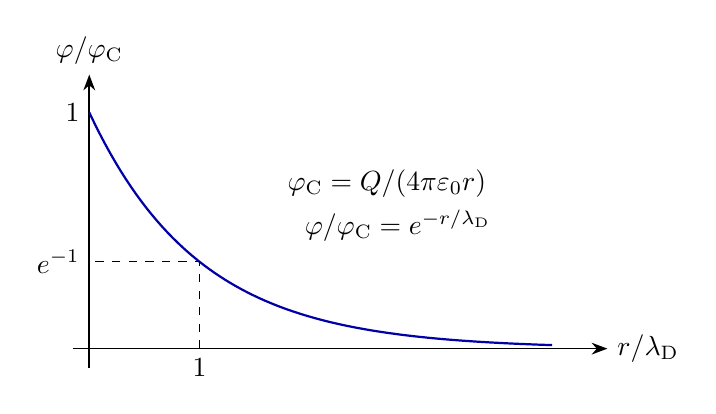
\begin{tikzpicture}[x=1.4cm,y=3cm]
\draw[arr] (-.15,0)--(4.7,0) node[right] {$r/\lambda_{\rm D}$};
\draw[arr] (0,-.08)--(0,1.16) node[above] {$\varphi/\varphi_{\rm C}$};
\draw[blue!65!black,thick,domain=0:4.2,samples=90] plot(\x,{exp(-\x)});
\draw[dashed] (1,0)--(1,.367879)--(0,.367879);
\node[below] at (1,0) {$1$}; \node[left] at (0,1) {$1$};
\node[left] at (0,.367879) {$e^{-1}$};
\node at (2.7,.7) {$\varphi_{\rm C}=Q/(4\pi\varepsilon_0r)$};
\node at (2.8,.52) {$\varphi/\varphi_{\rm C}=e^{-r/\lambda_{\rm D}}$};
\end{tikzpicture}
\end{document}
